Along with the contrast, the mean size of a speckle is an important figure of
merit for a speckle pattern, being connected to the underlying scattering
microstructure (surface roughness) and SPP transport therein.

As discussed earlier, a measurement of the speckle spot
size yields the transverse dimension of the coherent source
on the scattering surface.

%The mean speckle size, as a very
%important parameter of the speckle pattern, is of great
%importance to practical applications, e.g., measurement of
%the roughness of surfaces [2], detection of the scattering
%center concentration in a biological fluid [3], the particle
%aggregation [4] or determination of the optical thickness and
%the particle size in the scattering media [5]. Nevertheless,
%this paper is focused on determining the mean speckle size
%influenced purely by the properties of the light beam.

Following \name{Goodman}~\cite{goodman1975statistical} and
\name{Dainty}~\cite{dainty1975laser}, the size of a speckle is defined in
terms of the area of the normalized autocovariance function of the speckle
intensity pattern, $c_I(\Delta x, \Delta y)$.  The normalized autocovariance
function is likewise defined in terms of the autocorrelation $\Gamma_I(\Delta
x, \Delta y)$ by 
\begin{equation}
c_I(\Delta x, \Delta y) = \frac{\Gamma_I(\Delta x, \Delta y) - \bar{I}^2}{\bar{I}^2},
\end{equation}
and the autocorrelation is defined as
\begin{equation}
\Gamma_I(\Delta x, \Delta y) = \intinfty\intinfty I(x,y) \tilde{I}(x+\Delta x,y+\Delta y) \md x \md y.
\end{equation}
For computation on real images, the integral is replaced by a sum.  Taking
advantage of the Wiener–Khinchin theorem, the autocorrelation is simply the
Fourier transform of the power spectral density, vis.
\begin{equation}
\Gamma_I(\Delta x, \Delta y) = \ff{|I(x,y)|^2}(\Delta x, \Delta y)
\end{equation}
and thus  $c_I(\Delta x, \Delta y)$ can be efficiently calculated on a
computer\footnote{For example in MATLAB this is implimented with
\texttt{xcov(I,'coeff')}}.

With these definitions out of the way, the area of $c_I(\Delta x, \Delta
y)$ is simply its integral over $\Delta x$ and $\Delta y$
\begin{equation}
\mathscr{A}_c = \intinfty\intinfty c_I(\Delta x, \Delta y) \md \Delta x \md
\Delta y,
\label{eqn:spotsize1}
\end{equation}
or
\begin{equation}
\mathscr{A}_c \approx \approx\frac{{(\lambda z)}^2}{A}
\label{eqn:spotsize2}
\end{equation}
where $A$ is the illuminated area and $z$ is the observation distance.
Conceptually, \Equation{eqn:spotsize2} can be thought of as follows: the
difference between a ``bright'' spot and a ``dark'' spot in a speckle field
occurs when the scattering angle changes such that the optical path length
difference from the scattering center to the far field changes by
$\lambda$; here the speckle intensity is uncorrelated.

We have measured the speckle size in the experiment and found that, in
apparent contradiction with \Equation{eqn:spotsize}, the speckle size does
\textit{not} change with spot size for long range surface plasmons.  This
is shown in \Figure{fig:spotsize} for three different characteristic spot
sizes.  Here we have made a relative measurement of the scattering spot
size by fitting a Gaussian to its transverse dimension, and reporting the
full width at half maximum of that measurement as a measurement of the
actual spot size.
\begin{figure}[ht]
\centering
\import{includes/}{setpgfinc}
\import{speckle/figures/spotsize/}{spotsizefig}
%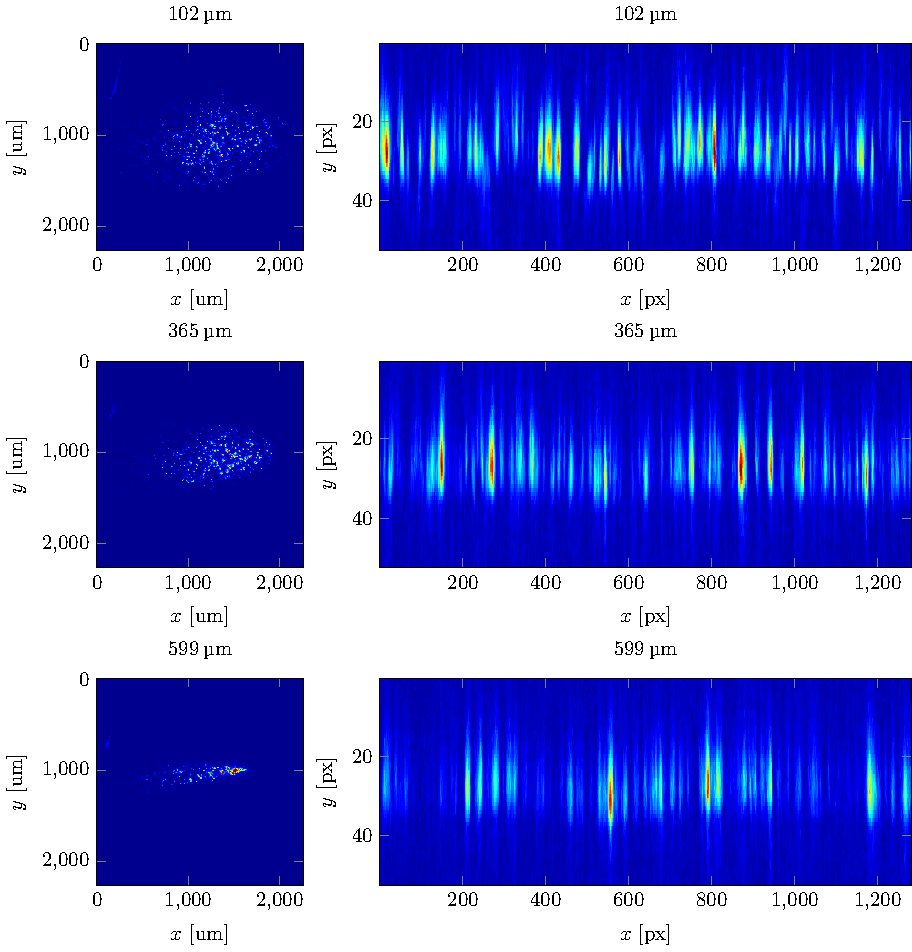
\includegraphics[keepaspectratio]{speckle/figures/spotsize/test.pdf}
\caption{Speckle size versus spot size for \SI{57}{\nano\meter} AuNPs adsorbed
onto a gold surface in a long range surface plasmon (symmetric) structure.}
\label{fig:spotsize}
\end{figure}
250um spot size prediction for all sizes

\begin{figure}[ht]
\centering
\import{includes/}{setpgfinc}
\import{speckle/figures/spotsize/}{test}
%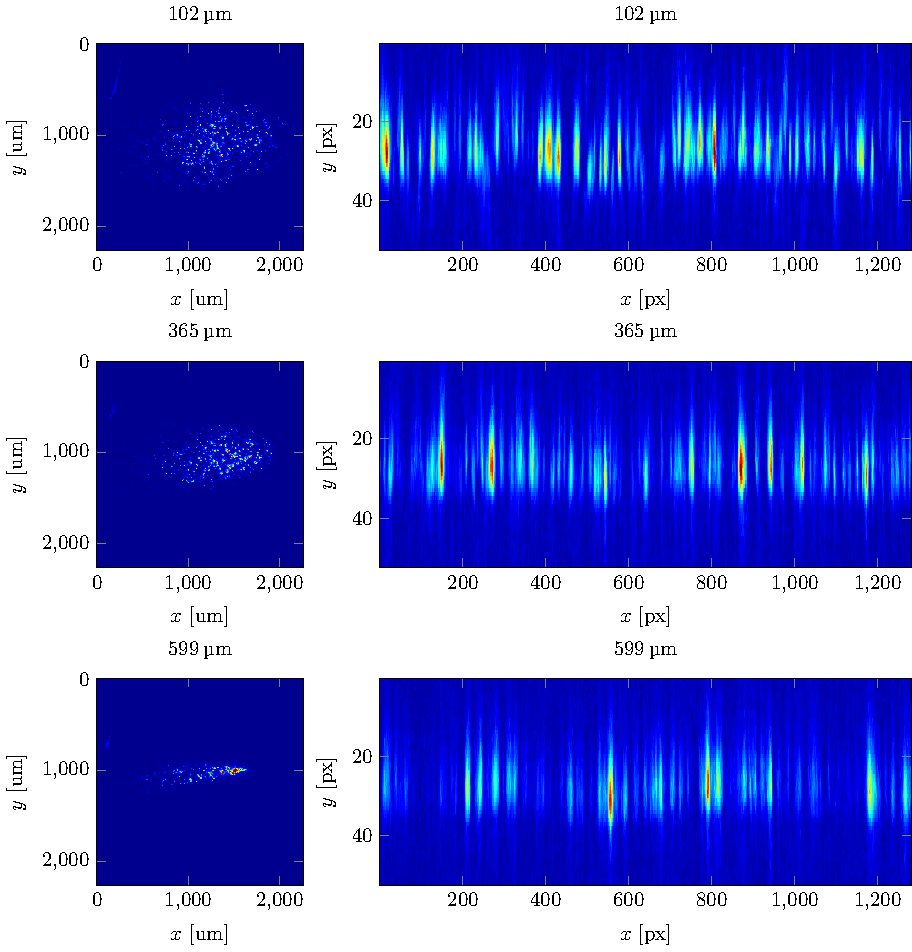
\includegraphics[keepaspectratio]{speckle/figures/spotsize/test.pdf}
\caption{Speckle size versus spot size for \SI{57}{\nano\meter} AuNPs adsorbed
onto a gold surface in a long range surface plasmon (symmetric) structure.}
\label{fig:spotsizewspeckle}
\end{figure}

%\caption{Speckle size versus spot size.  Inset images show an example of
%the raw spot size data from which the plot was computed.  Inset images are
%\SI{2.26x2.26}{\milli\meter} with major ticks at
%\SI{500}{\micro\meter} intervals.}

%MAKE SURE TO TALK ABOUT WHY NO ENHANCED SURFACE ROUGHNESS!  DO YOU HAVE ANY PICTURES?
